\documentclass[a4paper]{scrartcl}


\usepackage[utf8]{inputenc}
\usepackage[ngerman]{babel}
\usepackage{enumerate}
\usepackage{tikz}
\usepackage{fancyhdr}
\usepackage{lastpage}
\usepackage{verbatim}

\usepackage{listings}
\setlength{\parindent}{0mm}
\usepackage{graphicx}
\usepackage{amsmath}
\usepackage{algorithm2e}

\pagestyle{fancy}
\fancyhead[L]{SS 2017\\Joshua Hartmann}
\fancyhead[C]{Entwurf und Synthese von Eingebetteten Systemen\\Manfred Opel}
\fancyhead[R]{Blatt 5\\Nicolas Staller}

\fancyfoot[L]{}
\fancyfoot[C]{\thepage /\pageref{LastPage}}
\fancyfoot[R]{}

\renewcommand{\textheight}{700px}
\renewcommand{\footskip}{10px}
\newcommand*\xor{\mathbin{\oplus}}
\begin{document}	
	\section*{Aufgabe 1: Fragen zur Vorlesung}
	
	\begin{enumerate}[(a)]
		\item Der Arbiter im AHB Bus dient dazu die Bus Zugriffe der verschiedenen Master zu organisieren um sicherzustellen, dass jeweils nur ein Master den Bus zum gleichen Zeitpunkt verwendet.
		\item Der Adress- und Kontrollmultiplexer , gesteuert vom Arbiter, sorgt für korrekte Adressierung der Slaves. Der Master legt sein Adress- und Kontrollsignal an, der Arbiter steuert die entsprechenden Multiplexer so an, dass nach der Adressdekodierung die Daten am korrekten Slave ankommen.
		\item Design Constraints beschreiben bestimmte Einschränkungen an den Chip wie beispielsweise eine bestimmte Berechnungsgeschwindigkeit die für die Einsetzbarkeit notwendig ist, oder eine maximale Größe, die der Chip haben darf um eingebaut werden zu können.
		\item Nach Beendigung einer Berechnung und dem Zeitpunkt zu dem das Ergebnis der Berechnung am Register stabil verfügbar sein muss gibt es häufig eine zusätzliche Zeitspanne, den Slack, der dazu genutzt werden kann, dass zusätzliche geringen Verzögerungen bei der Berechnungen in Kauf genommen werden können ohne das gewünschte Ergebnis zu verändern.\\
		Damit kann man für diese Transferfunktion den Schlupf so nutzen, dass man z.B. eine kleinere Fläche nutzt und damit aber etwas länger für die Berechnung braucht.\\
		Durch eine statische Timing Analyse kann die Schlupfzeit berechnet werden. Dazu betrachtet man die Differenz des Delays der kombinatorischen Logik und der Dauer, bis der Eingang am Register stabil sein muss.
		
		\item Im allgemeinen hat der Operator bei den verschiedenen Operationen auch verschiedene Operanden und damit auch verschiedene Ergebnisse.\\
		Stünde durch Resource Sharing nur eine Einheit für diese Operation bereit, könnten nicht alle unterschiedlichen Ergebnisse berechnet werden. Denn man muss davon ausgehen, dass in einem Kontrollpfad potentiell alle Operationen parallel ausgeführt werden.
		
	\end{enumerate}
	\newpage
	\section*{Aufgabe 2: RTL-Synthese: Optimierungen in der Elaborationsphase}
	
	\begin{enumerate}[(a)]
	\item Unoptimierte Schaltung
	
	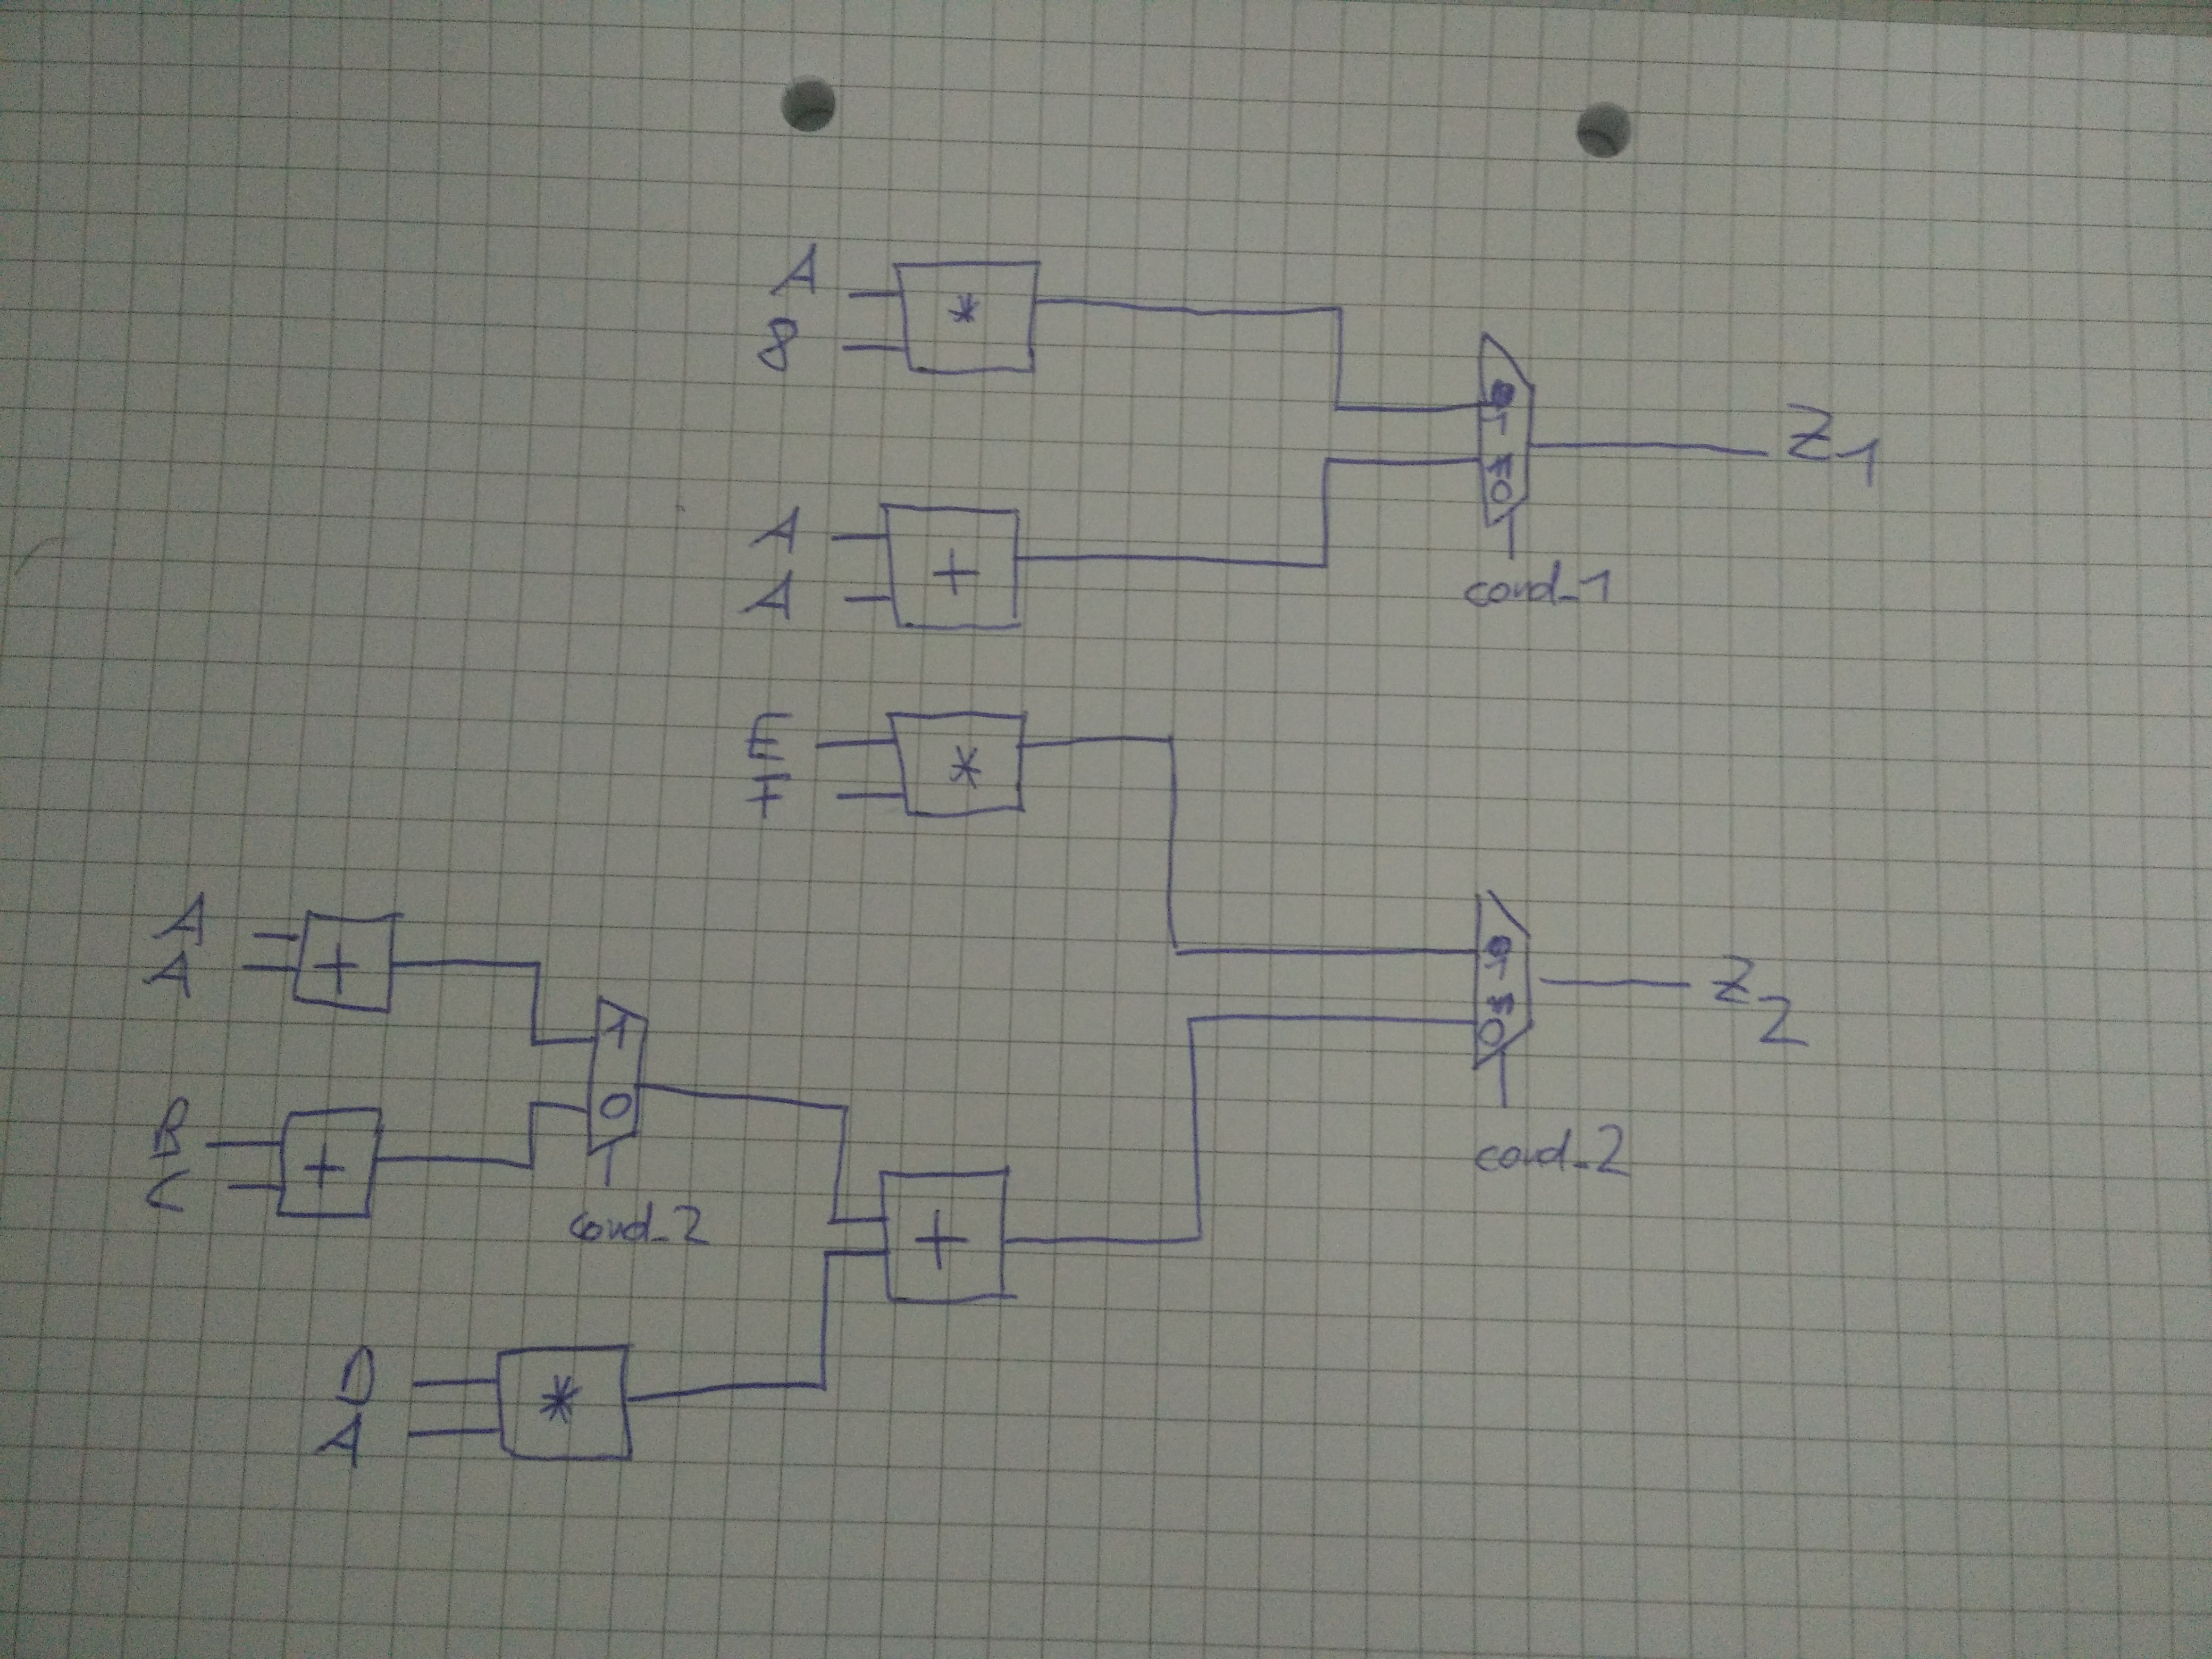
\includegraphics[width=\textwidth]{netlist}
	
	\item Benötigte Fläche:
	
	4 Addierer, 3 Multiplizierer, 3 Multiplexer\\
	$\implies$ 32 + 90 + 6 = 128 Flächeneinheiten
	
	\item Händisches Optimieren:\\
	
	Anmerkungen auch im Quelltext, aber Erläuterungen sind laut Blatt wohl im PDF gefordert.
	
	Reduktion von Multiplizieren:\\
	-A*8 ersetzt durch Shift um 3 nach links\\
	-Multiplikation E*F bzw D*A so gelöst, dass Operanden vorher durch Multiplexer bestimmt werden
	
	Reduktion von Addierern:\\
	-Z1 $<=$ A + A kann auch als Z1 $<=$ 2 * A bzw einen Shift um 1 nach links realisiert werden
	-für die Berechnung von Temp1 entsprechend gelöst wie bei der Multiplikation oben
	
	Reduktion von Shiftern:\\
	-in beiden Blöcken von cond1 ergibt sich letztendlich Z1 als Shift von A um 3 bzw 1 Stelle nach links, also wird die Shiftweite durch einen Multiplexer bestimmt
	
	
	
	
	\item Optimierte Schaltung
	
	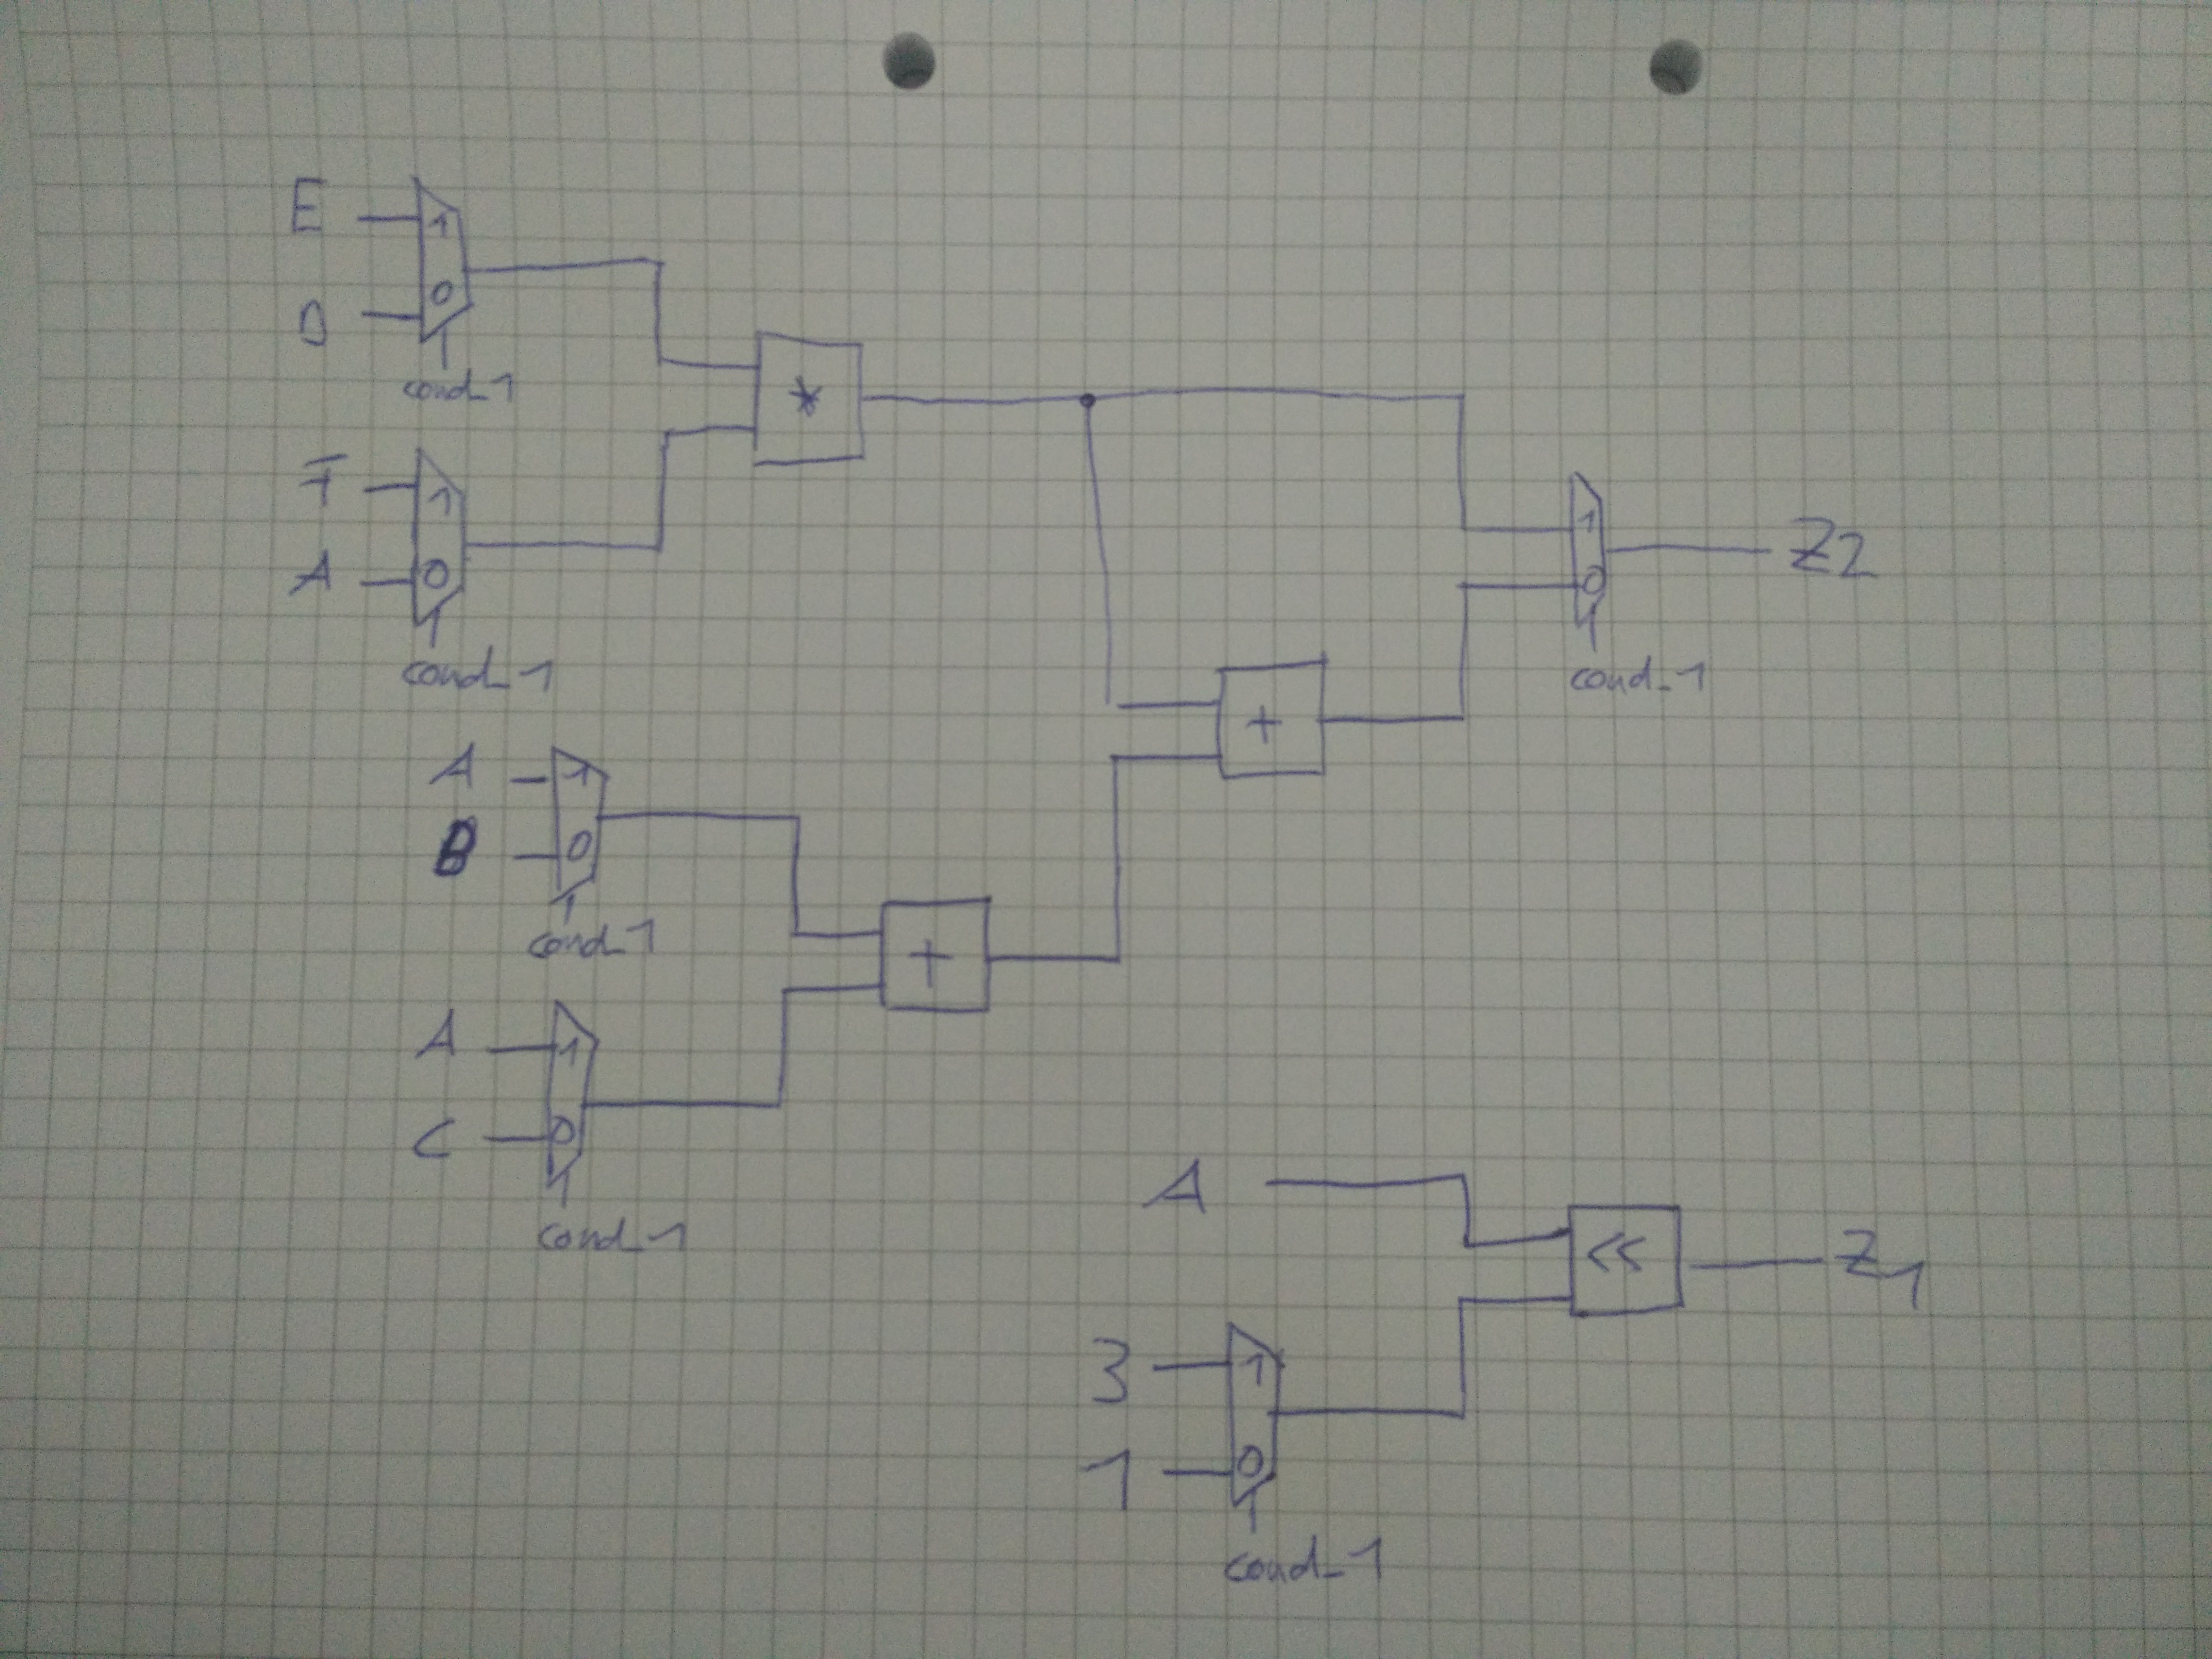
\includegraphics[width=\textwidth]{netlist_optimized}
	
	\item Benötigte Fläche:
	
	2 Addierer, 1 Multiplizierer, 4 Multiplexer, 1 Shifter\\
	$\implies$ 16 + 30 + 8 + 4 = 58 Flächeneinheiten
	
	\end{enumerate}

	
\end{document}

